\documentclass[a4paper, 10 pt, conference]{ieeeconf}
\overrideIEEEmargins
\usepackage{polski}
\usepackage[utf8]{inputenc}
\usepackage[T1]{fontenc}
\usepackage[english]{babel} 
\usepackage{graphicx}
\usepackage{amsmath}
\usepackage[T1]{fontenc}
\usepackage{textcomp}
\usepackage{listings}
\usepackage{xcolor}
\usepackage{amssymb}
\usepackage{url}
\usepackage{makecell}

\lstdefinestyle{mystyle}{
	backgroundcolor=\color{gray!5!white},   
	commentstyle=\color{green!50!black},
	keywordstyle=\color{magenta},
	numberstyle=\tiny\color{black!50!white},
	stringstyle=\color{purple},
	basicstyle=\footnotesize,
	breakatwhitespace=false,         
	breaklines=true,                 
	captionpos=b,                    
	keepspaces=true,                 
	numbers=left,                    
	numbersep=5pt,                  
	showspaces=false,                
	showstringspaces=false,
	showtabs=false,                  
	tabsize=2
}
\lstset{style=mystyle}

\usepackage{tikz}

\newcommand{\bb}{\textbf}
\DeclareMathOperator*{\argmax}{argmax}

\title{\LARGE \bf
Methods of feature extraction for broad and deep datasets
}

\author{ \parbox{2 in}{\centering Filip Guzy \\
        Wrocław University of Science and Technology\\
        {\tt\small 218672@student.pwr.edu.pl}}
        \hspace*{ 0.3 in}
        \parbox{2 in}{\centering Jędrzej Kozal \\
        Wrocław University of Science and Technology\\
        {\tt\small 218557@student.pwr.edu.pl}}
}

\begin{document}
\maketitle
\thispagestyle{empty}
\pagestyle{empty}

\selectlanguage{english}
\begin{abstract}

\end{abstract}

\section{Introduction}

Feature extraction (FE) is a fundamental part of Machine Learning. Its main responsibility it to make sure that our classifiers won't get tons of unnecessary data on their inputs. We can divide FE algorithms into two groups: statistical and non-statistical. The group of statistical methods contains algorithms like Principle Component Analysis (PCA) or Linear Discriminant Analysis (LDA). In the second group we can find methods based on artificial intelligence, such as Convolutional Neural Networks (CNN). 

Extracting particular features may help classifiers in making proper decisions, but in many cases it is not helpful for humans. When decision system is a black box, experts cannot use their intuition to predict the output, they also have no explanation why such decision was made. For example, it cannot be deduced why hospital diagnostic system assigned particular set of symptoms to the disease, or why loan request was rejected by the bank system.

Feature extraction methods can be straightly connected with the field of studies and analysed data. Therefore, many algorithms are composed to give the best performance for specific domain or particular type of data. With regard to this fact, in this article both basic FE methods and state-of-the-art solutions will be analysed and compared. The main focus will be put on the comparison of PCA, LDA, and CNN approaches by applying them to two datasets and testing their effectiveness on the selected classifiers.

\section{Related work}
PCA was introduced in 1901 paper \cite{PCA}. Currently it is one of the most popular feature extraction algorithms. It applies to many fields, especially to computer vision \cite{PCA_book}. Methods such as Robust PCA, Simplified PCA or Functional PCA were described in \cite{PCA_recent}. More insight into RPCA was given in \cite{RPCA}.

Linear Discriminant Analysis (LDA) was introduced in \cite{LDA} as a solution for binary classification problem. Important adjustments was made in \cite{multi_LDA}, that enabled usage of LDA for multi-class problem. Authors of \cite{LDA_recent} focused mainly on the problem of LDA for small sample size data, which is not relevant in case of this work, but it gives a good overview on the research done recently in this field.

Balanced local discriminant embedding (BLDE) and convolutional neural networks (CNN) as methods for spacial-domain and spectral-domain feature extraction were proposed in \cite{blde-cnn}. BLDE was used as a first part of the described hyperspectral images (HSI) classifier. Its task was to find a low-dimensional representation of classified images. Second part included CNN framework designed especially for extracting high level deep features. Extracted features were then stacked and input into Logistic Regression (LR) classifier. Usage of convolutional neural networks for feature extraction purposes was also proposed in \cite{cnn}. In this case, 3-D CNN model with combined regularization was used in spectral-spacial feature extraction. Comparison of 3-D CNN model with another deep learning based methods, like stacked autoencoder (SAE), deep brief network (DBN) or 2D-CNN-based method was described in \cite{cnn2}. Another CNN-based deep learning approach was shown in \cite{cnn3}. Proposed approach assumed usage of the special type of CNN architecture - Deep Pyramidal Residual Network. The specific part of this architecture were pyramidal bottleneck residual blocks of convolutional layers. It allows to gradually increase the feature map dimension at all convolutional layers, what leads to involving more locations as the network depth increases, balancing the workload among all units and preserving the time complexity on each layer. Another solution for improving spectral-spatial feature extraction was proposed in \cite{cnn4}. Traditional pooling layer of CNN was replaced with spatial pyramid pooling (SPP), what resulted in increasement of extraction effectiveness.

A different approach, based on propagation filter (PF), was presented in \cite{propagation-filter}. First, the PCA algorithm was used in order to reduce HSI dimensionality. Then, the extracted principal components were filtered with the PF. In the last step of the experiment, extracted and filtered spectral-spatial features were input into support vector machine (SVM) classifiers to test the effectiveness of the classification.

\section{Methods}

\subsection{Principle Component Analysis}
PCA allows to reduce dimensionality of selected dataset. It results in maximising the variance of dataset by the new basis of lower dimensional space. Let's suppose that space $\mathbb{R}^{M}$ is given and we want to lower its dimension to $D$. We want to find projection matrix that enables this transformation of space. We also want to lose as little information as possible. In this case, using PCA requires calculation of eigenvalues and eigenvectors of covariance matrix $S$ (or evaluation of scatter matrix $A$, and calculating eigenvalues and eigenvectors of $\frac{1}{N}AA^{T}$ matrix). $D$ eigenvectors, that correspond to the biggest eigenvalues are used as a basis of a new space. These eigenvectors point the directions of the biggest change of variance in data.  The same problem can be reframed as maximalization of variance while projecting on vector $\bb{u}$:

\begin{align}
	f(\bb{u}) &= \bb{u}^T S \bb{u} \\
	g(\bb{u}) &= 1 - \bb{u}^T \bb{u} = 0   \notag
\end{align}

where $f$ is variation while projecting on $\bb{u}$, and is additional constriction that yields $||\bb{u}||_{2} = 1$. The same can be formulated as Lagrangian:

\begin{align}
	\mathcal{L}(\bb{u}, \lambda) &= f(\bb{u}) - \lambda g(\bb{u}) \\
	    &= \bb{u}^T S \bb{u} - \lambda (1 - \bb{u}^T \bb{u})   \notag
\end{align}

and solved as optimization with the constrain problem. Please note that covariance matrix is symmetrical, i.e. it can be written as $S = Q \Lambda Q^{T}$, where $Q$ is an orthogonal matrix, and $\Lambda$ is a diagonal matrix with the real eigenvalues of $S$. According to this fact, finding new basis is always possible and new basis is always orthogonal.

Taking $\bb{u}_{n}$ as $n$-th eigenvector of covariance matrix, projection matrix $P$ can be written as:

\begin{align}
	P =
	\left( \begin{array}{l}
		\bb{u}_1^T \\
		\bb{u}_2^T \\
		\vdots	 \\
		\bb{u}_M^T
	\end{array} \right)
\end{align}

This matrix enables projection of any vector from $\mathbb{R}^M$ to $\mathbb{R}^D$.
More insight into the theory of PCA is given in \cite{Pattern_recognition}.

\subsection{Linear Discriminant Analysis}

LDA is a supervised dimensionality reduction algorithm, which aims to increase the linear separation of classes after projecting the orignal space. In order achieve this goal Fischer criterion is used:

\begin{equation}
    \argmax_{W} \frac{W^{T} S_{B} W}{W^{T} S_{W} W}
    \label{eq:Fischer_criterion}
\end{equation}

where $S_{B}$ is a between-class covariance, and $S_{W}$ is a within-class covariance. $W$ is a space that we are projecting on it. $S_{B}$ is defined as:

\begin{equation}
    S_B = \sum_{i} (\mu_{i} - \mu)(\mu_{i} - \mu)^{T}
\end{equation}

where $\mu_i = \frac{1}{n_{c_i}} \sum_{j=1}^{n_{c_j}} x_i$ is an average of samples from $i$-th class, and $\mu = \frac{1}{N} \sum_{j=1}^{N} x_j$ is an average of all samples. $S_B$ can be used to describe the distance between classes after performing projection on $W$:

\begin{align}
    (m_i - m)^2 &= (W^T \mu_i - W^T \mu)^2 \nonumber \\
                &= (W^T (\mu_i - \mu)(\mu_i - \mu)^T W \\
                &= W^T S_{B_i} W \nonumber
\end{align}

So, maximizing the nominator of the Fischer criterion results in best linear separability after projection to lower-dimension space.
$S_{W}$ is defined as:

\begin{equation}
    S_{W} = \sum_{i} A_{i}A_{i}^T
    \label{eq:SW}
\end{equation}

where $A_i$ is matrix of all samples $X_i$ from class $i$ reduced by $\mu_i$. $S_W$ is used to describe distance between samples of the chosen class and its mean after projection:

\begin{align}
    (W^{T} X_i - M_i)^2 &= (W^{T} X_i - W^{T} U_i)^2 \nonumber \\
                        &= W^{T} (X_i - U_i)(X_i - U_i)^T W \\
                        &= W^{T} S_{Wi} W \nonumber
\end{align}

where $U$ is a matrix of the same size as $X_i$ and all columns equal to $\mu_i$. Thus minimizing denominator of Fischers criterion causes an increasement of density samples from the same class. This enables easier linear separability.

Equation [\ref{eq:Fischer_criterion}] can be also formulated as:

\begin{equation}
    S_{W}^{-1} S_{B} W = \lambda W
\end{equation}

This corresponds to finding eigenvalues and eigenvectors of $S_{W}^{-1} S_{B}$ matrix. Choosing $D$ eigenvectors with the largest corresponding eigenvalues as a base of the new space $\mathbb{R}^D$ guaranties good linear separability between classes. 

\subsection{Convolutional Neural Networks}

Convolutional Neural Network is a special type of neural network that is mainly based on the mathematical operation called convolution and the mechanism of pooling. Convolution in general is a linear operation on two functions of a real valued arguments. Let's assume that $x(t)$ is a function output of some operation that is performed on data $t$, which is usually called input and $w(t)$ is another operation that is called kernel. $s(t)$ is a convolution output that is sometimes referred as a feature map. Then we can define convolution as below:

\begin{equation}
    s(t) = (x*w)(t) = \int x(a)w(t-a)da
\end{equation}

In case of feature extraction CNNs mostly operate on discrete data, so discrete convolution can be defined as:

\begin{equation}
    s(t) = (x*w)(t) = \sum_{\alpha=-\infty}^{\infty} x(a)w(t-a)
\end{equation}

For two-dimensional data, like image I and kernel K we define convolution as:

\begin{equation}
    s(i, j) = (I*K)(i, j) = \sum_m \sum_n I(i-m, j-n)K(m, n)
\end{equation}

According to \cite{Goodfellow-et-al-2016}, convolution operation is used in the first of  the three main stages of convolutional layer. This stage produces a set of linear activations by performing several convolutions in parallel. Second stage, sometimes called the detector stage, is responsible for passing linear activations through a nonlinear activation function, such as the rectified linear activation function. The last stage is based on a pooling function, which modifies the output of layer further. This function replaces the network output at certain location with a summary statistic of the nearby outputs. In some cases convolution, detector, and pooling stages are considered as separated network layers.

\section{Experimental settings}

\subsection{Data sets description}

\textsl{No free lunch theorems for Optimization} \cite{no-free-lunch} states that there is no general algorithm suited to solve all problems. Machine learning algorithms accuracy may depend on the application and the character of used data \cite{alppaydin}. For that reason datasets containing faces were chosen in order to perform comparison of selected extraction methods. These kind of datasets contain a lot of samples. Each sample contain many features, what suits the criterion of broad and deep datasets. Each pixel in image can be considered as a separate dimension. Chosen datasets are compared in table \ref{tab:datasets}.

\begin{table}[!h]
    \centering
    \caption{Comparison of datasets.}
    \begin{tabular}{|c|c|c|c|}
         \hline
         dataset & \thead{number of\\ images} & \thead{approximate\\ number of\\ images per subject} & source \\
         \hline
         Specs on Faces & 42,592 & >100 & \cite{afifi2017afif4} \\
         \hline
         JAFFE & 213 & 20 & \cite{JAFFE} \\
         \hline
         Caltech Faces 1999 & 450 & 16 & \cite{CaltechFaces} \\
         \hline
         Georgia Tech & 750 & 15 & \cite{georgia_tech_face_database} \\
         \hline
         UMist-Faces & 576 & 30 & \cite{UMist-Faces} \\
         \hline
         Stirling faces & 312 & 9 & \cite{Stirling_faces} \\
         \hline
         VidTIMIT & 94600 & >100 & \cite{VidTIMIT} \\
         \hline
         muct & 3755 & 15 & \cite{Milborrow10} \\
         \hline
         yale & 330 & 22 & \cite{yale} \\
         \hline
         AT\&T Database & 400 & 10 & \cite{TheDatabaseOfFaces} \\
         \hline
         MIT-CBCL  & 2000 & >100 & \cite{FaceRecognitionDatabase} \\
         \hline
         Essex Collection & 7900 & 20 & \cite{essex} \\
          \hline
    \end{tabular}
    \label{tab:datasets}
\end{table}

All images in chosen datasets contain varying lightning conditions, emotion expressions, face angles, varying ethnicity, sex and age of the subjects. Pictures were converted to the grayscale before performing feature extraction. 

\subsection{Experiment description}

PCA, LDA, and CNN-based feature extraction methods and classifiers were trained using same training set. Models were evaluated using 10-fold stratified cross validation, which guarantee, that both training and test sets contain proportional number of images for each class. Accuracy was chosen as measure. The results for given classifier were given as an fold-wise average of all results obtained via cross validation.

Classifiers used for comparison of feature extraction methods were Neural Network and Svc. All classifiers hyperparameters were fixed during whole experiment. Searching for the best hyperparameters for each dataset and extraction method could compromise gathered results of experiment.

Analysis of results was performed using Friedman test with Nemenyi post-hoc test, as suggested in \cite{demsar}.

\section{Results}

Tests were performed separately for SVC and MLP classifiers for all FE methods. Obtained accuracy and training time were presented in below tables and plots.

Nemenyi test ranks perfomernce of algithms for each dataset, then calculates mean of ranks for algorithms. Means are tested using Tukey test (to be more precise: diffrence of means are compared to standard error), to check if there is singnificant diffrence in performance over multiple datasets. In case of 3 datasets there are only 3 ranks, that can be obtained. Each rank for chosen algorithm and dataset can take value 1, 2 or 3, therefore diffrence between mean ranks will not obtain large value (in fact maximal diffrence between mean ranks is 2). Significant diffrence will be noted by Neymani test between two algrithms achiving mostly ranks 1 or 3. This is clear limitation of post hoc analysis in this case. Suppose we got two algorithms with good performence (algorithms A and B) and one algrithm with poor performance (algorithm C). Algorithm A is slightly beeter then algorithm B, therefore obtains more frequently rank 3. In this case due to comparing only avrage ranks sigginifcant diffrence between algorithm A and C will be reported, and no significant diffrence will be reported for algorithms B and C. This was taken into consideration in further analysis of results.

%During testing some problems occured. For some dataset with large number of images Python virtual machine run out of memory on machine with 8 Gb RAM. This happend during computing eigenvalues and eigenvectors of $S_W$ matrix (when establishing within variance) while performing LDA for vidtimit dataset. $A_i$ (see equation \ref{eq:SW}) contains only images for $i$-th class. Maximal number of images for one class in vidtimit is 2644. Images are stored using 8 bit uint type. All images are converted to greyscale, so there is one 8 bit unsigned int per pixel. Sckit-learn use SVD implementation from numpy to establish eigenvalues and eigenvectors of $S_W$. In theory memory needed for storage of SVDs decomposition matrixes given all previous asumptions is aproximatly 0.25 Gb, which should not be problem. Numpy utilises Lapack library for SVD computation. Lapack is linear algebra library written in Fortran. There is little known about alorithms used to perform SVD in Lapack, therefore reason of raising MemoryError cannot be established.
%How the problem was solved? T.B.C.


\subsection{Results for SVC}


\begin{table}[!h]
    \centering
    \caption{Comparison of avrage accuracy of Svc classifier for chosen FE methods and datasets}
    \begin{tabular}{|r|l|l|l|}
  \hline
    & CNN & LDA & PCA \\
  \hline
  att: & 0.98 & 0.97 & 0.55 \\
  \hline
  caltec: & 0.99 & 0.99 & 0.94 \\
  \hline
  georgia & 0.86 & 0.70 & 0.10 \\
  \hline
\end{tabular}

    \label{table:svm_acc_comparison}
\end{table}

\begin{table}[!h]
    \centering
    \caption{Comparison of avrage time of traning Svc classifier for chosen FE methods and datasets}
    \begin{tabular}{|r|l|l|l|}
  \hline
    & CNN & LDA & PCA \\
  \hline
  att: & 9.84 & 0.66 & 3.08 \\
  \hline
  hands digits: & 38.88 & 5.89 & 5.17 \\
  \hline
  caltec: & 10.72 & 0.42 & 1.20 \\
  \hline
\end{tabular}

    \label{table:svm_fit_time_comparison}
\end{table}

\begin{table}[!h]
    \centering
    \caption{Comparison of p-values and F-values for Friedman test for Svc classifier}
    \begin{tabular}{|r|l|}
  \hline
    & values \\
  \hline
  p-value & 3.678794e-01 \\
  \hline
  value of statistic F & 2.00 \\
  \hline
\end{tabular}

    \label{table:svm_pvalues}
\end{table}

\begin{table}[!h]
    \centering
    \caption{Pvalues of Neymani posthoc tests .}
    \begin{tabular}{|c|c|c|c|}
         \hline
          & CNN & LDA & PCA \\
         \hline
         CNN &  - &  0.128 &  0.003 \\
         \hline
         LDA &  - & - &  0.381 \\
         \hline
         PCA &  - & - & - \\
         \hline
    \end{tabular}
    \label{tab:svm_posthoc_pvalues}
\end{table}

\begin{figure*}[!h]
    \centering
    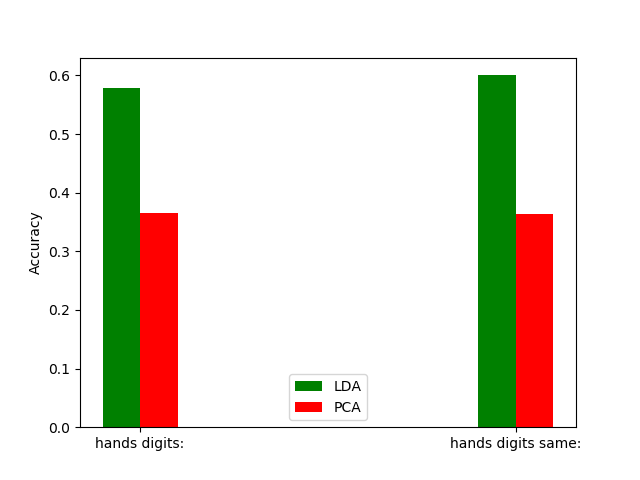
\includegraphics[scale=0.875]{images/Svm_accuracy_comparison.png}
    \caption{Comparison of avrage accuracy of Svc classifier for chosen FE methods and datasets}
    \label{fig:svm_acc_comparision}
\end{figure*}

\begin{figure*}[!h]
    \centering
    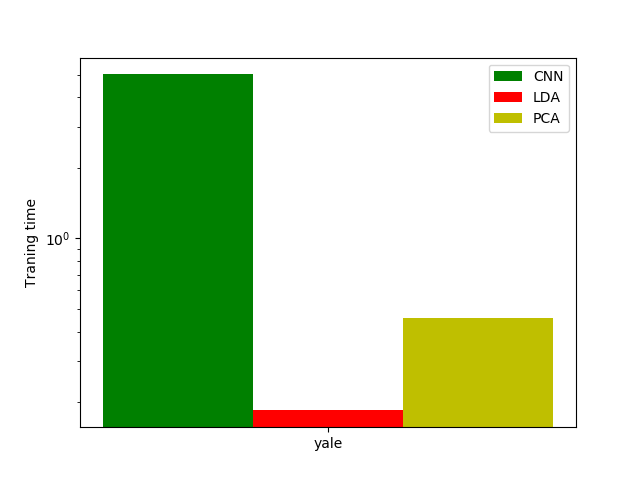
\includegraphics[scale=0.875]{images/Svm_fit_time_comparison.png}
    \caption{Comparison of avrage time of traning Svc classifier for chosen FE methods and datasets}
    \label{fig:svm_fit_time_comparision}
\end{figure*}

According to obtained results, null hypothesis of Friedmann test was rejected with $\alpha = 0.05$ (see Table \ref{table:svm_pvalues}). 
Results of post-hoc Nemenyi tests for FE methods similarity were shown in Table \ref{tab:svm_posthoc_pvalues}. Ranks obtained in post hoc testing for CNN, LDA and PCA were correspondingly 2.625, 2.125 and 1.25. 


\subsection{Results for MLP}


\begin{table}[!h]
    \centering
    \caption{Comparison of avrage accuracy of MLP classifier for chosen FE methods and datasets}
    \begin{tabular}{|r|l|l|l|}
  \hline
  \rowcolor{Gray}
  dataset & CNN & LDA & PCA \\
  \hline
  yale & 0.87 & 0.95 & 0.74 \\
  \hline
  essex & 0.98 & 0.90 & 0.91 \\
  \hline
  vidtimit & 1.00 & 1.00 & 1.00 \\
  \hline
  att & 0.94 & 0.97 & 0.82 \\
  \hline
  caltec & 0.99 & 1.00 & 0.88 \\
  \hline
  georgia & 0.84 & 0.79 & 0.55 \\
  \hline
  jaffe & 1.00 & 0.99 & 0.95 \\
  \hline
  mit & 1.00 & 0.97 & 0.99 \\
  \hline
  muct & 0.89 & 0.77 & 0.45 \\
  \hline
  specs-on-faces & 0.81 & 0.71 & 0.73 \\
  \hline
  stirling & 0.96 & 0.89 & 0.74 \\
  \hline
  umist & 0.99 & 0.99 & 0.95 \\
  \hline
\end{tabular}

    \label{table:NN_acc_comparison}
\end{table}

\begin{table}[!h]
    \centering
    \caption{Comparison of avrage time of traning MLP classifier for chosen FE methods and datasets}
    \begin{tabular}{|r|l|l|l|}
  \hline
  \rowcolor{Gray}
  dataset & CNN & LDA & PCA \\
  \hline
  yale & 5.82 & 0.84 & 0.77 \\
  \hline
  essex & 187.58 & 218.86 & 21.70 \\
  \hline
  vidtimit & 709.47 & 970.20 & 65.94 \\
  \hline
  att & 15.57 & 2.05 & 1.69 \\
  \hline
  caltec & 16.12 & 2.03 & 1.54 \\
  \hline
  georgia & 34.72 & 5.38 & 3.23 \\
  \hline
  jaffe & 11.90 & 0.98 & 0.92 \\
  \hline
  mit & 134.90 & 63.97 & 12.45 \\
  \hline
  muct & 325.28 & 41.34 & 39.81 \\
  \hline
  specs-on-faces & 82.67 & 17.98 & 13.00 \\
  \hline
  stirling & 21.33 & 3.73 & 2.38 \\
  \hline
  umist & 27.42 & 2.93 & 2.78 \\
  \hline
\end{tabular}

    \label{table:NN_fit_time_comparison}
\end{table}

\begin{table}[!h]
    \centering
    \caption{Comparison of p-values and F-values for Friedman test for MLP classifier}
    \begin{tabular}{|r|l|}
  \hline
    & values \\
  \hline
  p-value & 0.003 \\
  \hline
  value of statistic F & 11.87 \\
  \hline
\end{tabular}

    \label{table:NN_pvalues}
\end{table}

\begin{table}[!h]
    \centering
    \caption{Pvalues of Neymani posthoc tests for MLP classifier.}
    \begin{tabular}{|c|c|c|c|}
         \hline
          & CNN & LDA & PCA \\
         \hline
         CNN &  - &  0.438 &  0.002 \\
         \hline
         LDA &  - & - &  0.081 \\
         \hline
         PCA &  - & - & - \\
         \hline
    \end{tabular}
    \label{tab:NN_posthoc_pvalues}
\end{table}

\begin{figure*}[!h]
    \centering
    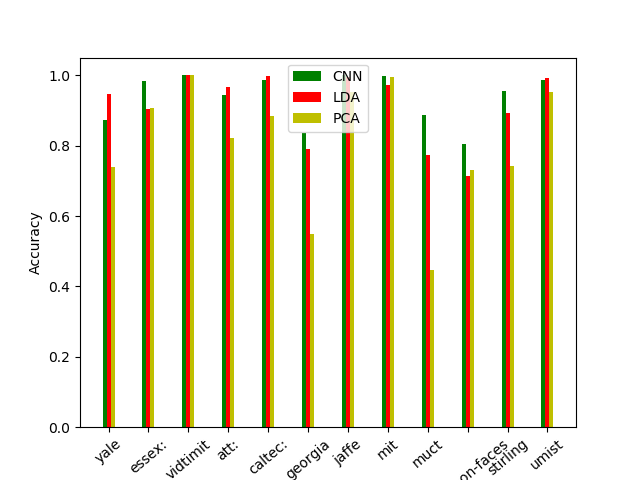
\includegraphics[scale=0.875]{images/NN_accuracy_comparison.png}
    \caption{Comparison of avrage accuracy of MLP classifier for chosen FE methods and datasets}
    \label{fig:NN_acc_comparision}
\end{figure*}

\begin{figure*}[!h]
    \centering
    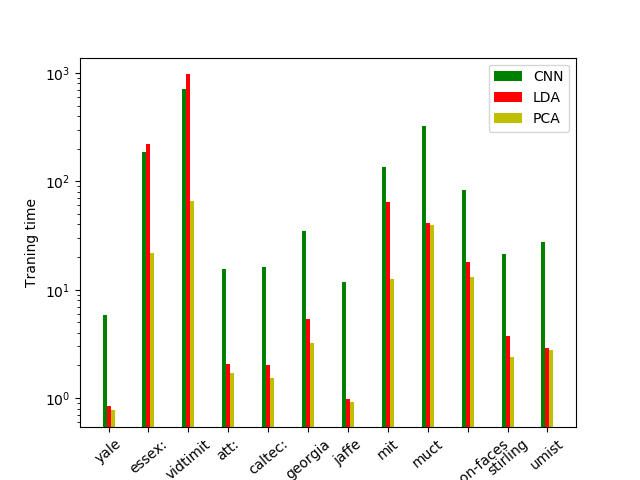
\includegraphics[scale=0.875]{images/NN_fit_time_comparison.png}
    \caption{Comparison of avrage time of traning MLP classifier for chosen FE methods and datasets}
    \label{fig:svm_fit_time_comparision}
\end{figure*}

Ranks obtained with post hoc tests: 2.625 2.125 1.25.


\section{Conclusions}


\bibliographystyle{plabbrv}
\bibliography{bibliography}

\end{document}